\chapter{Modelling the thermal conductivity of lower mantle minerals} % Main chapter title

\label{Chapter4} % Change X to a consecutive number; for referencing this chapter elsewhere, use \ref{ChapterX}

%-----------------------------------------------------------
\section{Simulating the effect of atomic impurities}
%-----------------------------------------------------------

The lower mantle is not uniform in terms of composition, featuring bridgmanite, post-perovskite, and periclase, among others. The composition can vary within these mineral archetypes, significantly the concentration of iron impurities. Magnesium is replaced with iron in 
\mgsios and MgO compositions, leading towards \fesios and FeO endmembers. Aluminium can similarly be subsituted for Magnesium (((REF))).

Impurities reduce \tcs by providing more opportunities for phonon scattering events. An impurity is an irregularity to a propagating phonon, much like a speedbumb to a car. They have different properties to the atoms the phonon expects to meet from crystal regularity, namely mass and their bonds with neighbouring atoms. It is for this reason that the \tcs of a solid solution is lower at intermediate compositions than at the endmembers. Even if one endmember has lower \cs than the other, an irregular mix of the two can produce even lower values.

%---------------------------------------
\subsection{How does iron behave?} 
%---------------------------------------

I use two methods to add iron impurities to classical molecular dynamics simulations. The first approach is to simply create a magnesium atom with the mass of an iron atom, without changing any coefficients of the interatomic potentials from \citet{Oganov2000}. Despite being an obviously "quick and dirty" method, this is a reasonable first-order approximation(((PROVE IT!?))). As the variation in mass number from Mg to Fe is so drastic (24 to 56, a 133\% increase), it is likely to change the behaviour of the system more than a subtle change in the atomic interactions.

The second approach to add Fe into the \mgsios system is to fit interatomic potentials, as well as using the aforementioned mass change for a more realistic model. We adapt the \citet{Oganov2000} \mgsios Buckingham interatomic potential ($U$) to include the Fe-O interation. We must determine two short-range potential parameters, $b$ and $\rho$, shown in Eq. 11 from \citet{Oganov2000},

\begin{equation}
U_{ij}\left ( R_{ij} \right ) = \frac{z_{i}z_{j}}{R_{ij}} + b_{ij}\ \textup{exp}\left ( - \frac{R_{ij}}{\rho_{ij}} \right ) - \frac{c_{ij}}{{R_{ij}}^{6}}, \label{og_buck}
\end{equation}

where $ij$ refers to an atom pair, $R$ is interatomic distance, $z$ is atomic charge, and $c$ relates to the Van der Waals force (zero for non O-O interactions). We determine $\rho$ in the same fashion as \citet{Oganov2000}, calculated from the atomic first ionisation potentials,

\begin{equation}
\rho_{ij} = \frac{1.85}{\sqrt{I_{i}}+\sqrt{I_{j}}}.  \label{urusov}
\end{equation}

$b$ is constrained using the GULP code \citep{Gale1997}, using the calculated $\rho$ value for Fe-O. We fit to the elasticity results of \citet{Parise1990}, an experimental study of (Mg$_{0.9}$,Fe$_{0.1}$)SiO$_3$ bridgmanite up to 433~K. Despite potential fitting being an improvement on solely changing mass (((PROVE IT!?))), it is still not perfect as the charge of our fitted Fe is not varied from the original Mg.

!!! Validate potentials

!!! Difference in results between Fe-approaches?



%---------------------------------------
\subsection{Where do the impurities go?} 
%---------------------------------------

Iron is substituted with magnesium into the bridgmanite atomic structure. The unit cell contains 4~Mg atoms, and the smallest direct method cell I employ is a 6x2x2 supercell. Therefore the smallest amount of iron that can be added is 1/96 atoms, a concentration just over 1\%. A simple script (((INCLUDE IN APPENDIX, MENTION MATLAB?))) is used to modify LAMMPS input files, randomly selecting a specified proportion of Mg atoms to be replaced with Fe. When a Mg atom changes to Fe, its mass and interatomic potential properties change. 

Due to the microscopic nature of the system, we do not want all of the added iron to be clumped together, especially in a heat source/sink region (((ELABORATE?))). To avoid this we order Mg atoms by length along supercell, and change a single atom every so many. For example, changing 1/4 atoms is different to changing 24/96. The latter has a higher variance in Fe per unit length, and the former chooses one atom to swap for every four along the system. After iron is added, the standard direct method or Green-Kubo workflow is followed.


%-----------------------------------------------------------
\section{Making the model}
%-----------------------------------------------------------

Due to uncertainty in the lower mantle's compositional distrubution, properties like \tcs are averaged considering the relative abundance of each mineral component. There are also endmember relations to consider within each mineral, the concentration of impurities, and mineral phase transitions.  

A simple weighted average can be taken to combine the contributions of individual minerals, whereas mixing between endmembers is not as linear. \citet{Ohta2017} provide an equation for interpolating \cs between compositional endmembers, specifically (Mg,Fe)O (ferro)periclase. I apply it to (Mg,Fe)SiO$_3$ perovskite [[[PRESUMABLY ALSO WORKS FOR bdg<->p-Pv?]]]. 

\citet{Okuda2017} present a temperature scaling relation for bridgmanite, which I additionally apply to the Fe-endmember. By having temperature-dependent values I am able to obtain an equation that gives \tcs as a function of both temperature and composition, for a given (studied/fit?) endmember pair.

%---------------------------------------
\subsection{Fitting the data} 
%---------------------------------------

[Equations from \cite{Ohta2017} (eq. 7,8,9), and \cite{Okuda2017} (eq. 5)]

I want to determine lattice thermal conductivity as a function of temperature and composition, 
using calculated and fit constants. For the method I will use I need to know how the conductivity of endmember minerals changes with physical conditions. In order to keep temperature the only dependent variable, I will scale volume linerarly with temperature [FIGURE]. At this point I can scale the conductivity of an endmember with temperature within the fitted range \citep{Okuda2017}.

Considering \citet{Ohta2017} the linear interpolation between the conductivities two endmembers can be perturbed, forming the trough characteristic of varying composition. While \fesios generally has a lower \tcs than \mgsio, the minimum is located at an intermediate composition. The effect of impurity scattering is larger than inherent changes due to chemistry.
    
%-------------------
\subsubsection{Compositional dependence}
%-------------------
\cite{Ohta2017}\\
* = already cited somewhere above\\

Ohta eq. 7 
\begin{equation}%-----
\kappa_{latt}=\kappa_{i}\left ( \frac{\omega_{0}}{\omega_{M}} \right )arctan\left ( \frac{\omega_{M}}{\omega_{0}} \right )
\label{eq.ohta7}
\end{equation}%-------
\\ $\kappa_{latt}$ - output conductivity as function of t \& x (\wmk), considering mineral specific parameters\\
$\kappa_{i}$ - the composition-dependent conducitivity, if it were linearly interpolated between endmembers (\wmk)\\
$\omega_{0}/\omega_{M}$ - temperature-dependent parameter to perturb $\kappa_{i}$, to create the "trough" trend in composition-dependent conductivity\\
$\omega_{0}$ - \enquote{\textit{the phonon frequency where the intrinsic mean free path is equal to that due to solute atoms}}\\
$\omega_{M}$ - \enquote{\textit{the phonon frequency corresponding to the maximum of the acoustic branch of the phonon spectrum}}\\

Ultimately this is the equation we are trying to solve. The two components $\kappa_{i}$ and $\omega_{0}/\omega_{M}$, are both temperature and composition-dependent. $\kappa_{i}$ gives the compositionally-weighted average conductivity, a linear interpolation between endmembers at a certain temperature. $\omega_{0}/\omega_{M}$ controls the conductivity decrease due to the impurity effect, the magnitude of which depends on the temperature and composition of interest.\\

Ohta eq. 8 
\begin{equation}%-----
\left ( \frac{\omega_{0}}{\omega_{M}} \right )^{2}=\frac{\chi^{T}}{C\left ( 1-C \right )}  
\label{eq.ohta8}
\end{equation}%-------
\\ *$\omega_{0}/\omega_{M}$ - temperature-dependent parameter to perturb $\kappa_{i}$, to create the "trough" trend in composition-dependent conductivity\\
*$\omega_{0}$ - \enquote{\textit{the phonon frequency where the intrinsic mean free path is equal to that due to solute atoms}}\\
*$\omega_{M}$ - \enquote{\textit{the phonon frequency corresponding to the maximum of the acoustic branch of the phonon spectrum}}\\
$\chi^{T}$ -temperature-dependent parameter to \dots ??? \\
$\chi$ - \enquote{\textit{a constant}}\dots\\
$T$ - temperature of interest (K, default data fit between 1000 - 5000 K, but extrapolation should be reasonable)\\                    
$C$ - composition mix of interest (dimensionless, values between 0 and 1)\\

The equation that splits $\omega_{0}/\omega_{M}$ into its temperature and composition-dependent components, where $\chi$ is a temperature-dependent variable. $C\left ( 1-C \right )$ is largest when $C=0.5\ or\ 50\%$, relating to the shape of the trough formed by this fit.\\

$\chi^{T}$ scaling 
\begin{equation}%-----
\chi^{T}=A T^{B}
\label{eq.chi_scale}
\end{equation}%-------
\\ *$\chi^{T}$ -temperature-dependent parameter to \dots ??? \\
*$\chi$ - \enquote{\textit{a constant}}\dots\\
*$T$ - temperature of interest (K, default data fit between 1000 - 5000 K, but extrapolation should be reasonable)\\                    
$A$ - coefficient in $\chi^{T}$ variation with temperature\\
$B$ - exponent in $\chi^{T}$ variation with temperature\\

$\chi$ is a temperature-dependent variable, but a plot of $\chi$ against $T$ has no obvious trend. A simple power law can be fit to $\chi^{T}$ against $T$ however, with a coefficient $A$ and exponent $B$.\\

Ohta eq. 9 
\begin{equation}%-----
\kappa_{i}=\left ( 1-C \right )\kappa_{MgSiO_{3}}+C\ \kappa_{FeSiO_{3}}
\label{eq.ohta9}
\end{equation}%-------         
\\ *$\kappa_{i}$ - the composition-dependent conducitivity, if it were linearly interpolated between endmembers (\wmk)\\
*$C$ - composition mix of interest (dimensionless, values between 0 and 1)\\
$\kappa_{MgSiO_{3}}$ - temperature and volume-dependent conductivity for Mg endmember (\wmk)\\
$\kappa_{FeSiO_{3}}$ - temperature and volume-dependent conductivity for Fe endmember (\wmk)\\

An equation that describes the conductivity of an endmember mix, assuming the relation is a simple weighted mean. $C$, in this case specifically, is the proportion of Fe atoms swapped into the system for Mg. The actually dependence of conductivity with composition is more complicated on the atomic scale, this intermediate average value adjusted in Eq.~\ref{eq.ohta7} \citep[][Eq. 7]{Ohta2017}. \\

%-------------------
\subsubsection{Temperature dependence}
%-------------------

\cite{Okuda2017}\\

Okuda eq. 5 

\begin{equation}%-----
\kappa_{adj}=\kappa_{ref}\left ( \frac{\rho}{\rho_{ref}} \right )^{g}\left ( \frac{T_{ref}}{T} \right )^{a}
\label{eq.okuda5}
\end{equation}%-------
\\ $\kappa_{adj}$ - temperature and density-dependent conductivity of an endmember (\wmk)\\
$\kappa_{ref}$ - reference conducitivty\\
$T_{ref}$ - reference temperature\\
$a$ - exponent controlling temperature-dependent conducitvity of an endmember\\
$\rho_{ref}$ - reference density\\
$g$ - exponent controlling density-dependent conducitvity of an endmember\\

\citet{Okuda2017} present a model for density and temperature-dependent conductivity (actually from Manthilake 2011, REF???), which utilises exponents obtained from fitted data. A reference value is scaled to infer conductivity at the conditions of interest.\\



Okuda eq. 5 modified

\begin{equation}%-----
\kappa_{adj}=\kappa_{ref}\left ( \frac{T_{ref}}{T} \right )^{a}\left ( \frac{V_{ref}}{V} \right )^{h}
\label{eq.okuda_mod}
\end{equation}%-------
\\ $T_{ref}$ - temperature at which reference conductivity is calculated (K)\\
$T$ - temperature of interest to interpolate (K, default data fit between 1000 - 5000 K, but extrapolation should be reasonable)\\   
$V_{ref}$ - reference volume of an endmember (E-30 m$^3$)\\
$V$ - temperature-dependent volume of an endmember (E-30 m$^3$)\\
$h$ - exponent controlling volume-dependent conducitvity of an endmember\\

I adjust Eq.\ref{eq.okuda5} to consider volume instead of density, where density and volume are inversely proportional.










Volume scaling ($y=mx+c$)  
\begin{equation}%-----
V=\frac{\partial V}{\partial T} T+V_{T_{0}}
\label{eq.vol_scale}
\end{equation}%-------     
\\ *$V$ - temperature-dependent volume of an endmember (E-30 m$^3$)\\          
${\partial V}/{\partial T}$ - fit gradient, change of volume with temperature (E-30 m$^3$/K)\\
*$T$ - temperature of interest (K, default data fit between 1000 - 5000 K, but extrapolation should be reasonable)\\
$V_{T_{0}}$ - intercept volume for T=0~K (E-30 m$^3$)\\

I take Eq.~\ref{eq.okuda5} \citep[][Eq. 5]{Okuda2017} a step further, by obtaining $V$ in terms of $T$. This dependence is effectively linear over the temperatures considered, meaning Eq.~\ref{eq.ohta7} \citep[][Eq. 7]{Ohta2017} is dependent solely on temperature, composition, and fit or calculated constants.


%-----------------------------------------------------------
\section{Results}
%-----------------------------------------------------------
Taking Green-Kubo results at the full range of lower mantle temperatures (1000-5000~K) and CMB pressure (136~GPa), I fit Equation \ref{eq.okuda5} to obtain conductivity as a function of temperature for Mg and Fe silicate perovskite endmembers (Figure \ref{fig:kappa-temp_01}).
\begin{figure}[h!]
  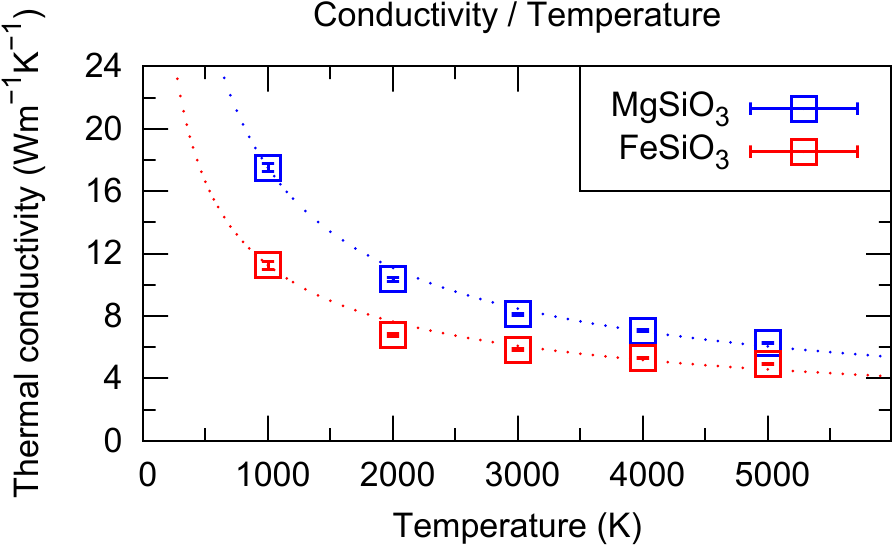
\includegraphics[width=\linewidth]{Figures/k-t_all_01.png}
  \caption{Data points are GK conductivity results, dotted line is the fit from Equation \ref{eq.okuda5}.}
  \label{fig:kappa-temp_01}
\end{figure}

We also consider the effects of variable Mg:Fe across the same temperatures and pressures (Figure \ref{fig:kappa-comp_01}). Conductivity decreases sharply as Fe is introduced and reaches a plateau around intermediate compositions, then increases towards 100\% Fe. 

\begin{figure}[h!]
  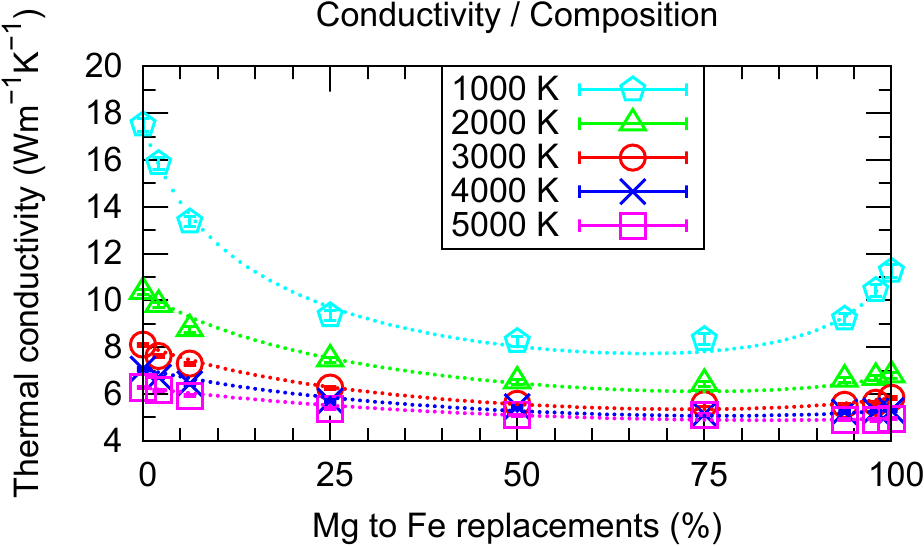
\includegraphics[width=\linewidth]{Figures/k-c_all_01.png}
  \caption{CAPTION}
  \label{fig:kappa-comp_01}
\end{figure}

A simple interpolation between endmember conductivities is insufficient, the presence of a compositional mix has an effect. This effect is itself temperature-dependent, the trough-like trend flattens with increasing temperature. These temperature and compositional dependences can be combined, allowing conductivity to be determined for a range of possible CMB conditions (Figure \ref{fig:kappa-temp-comp_01}). 

\begin{figure}[h!]
  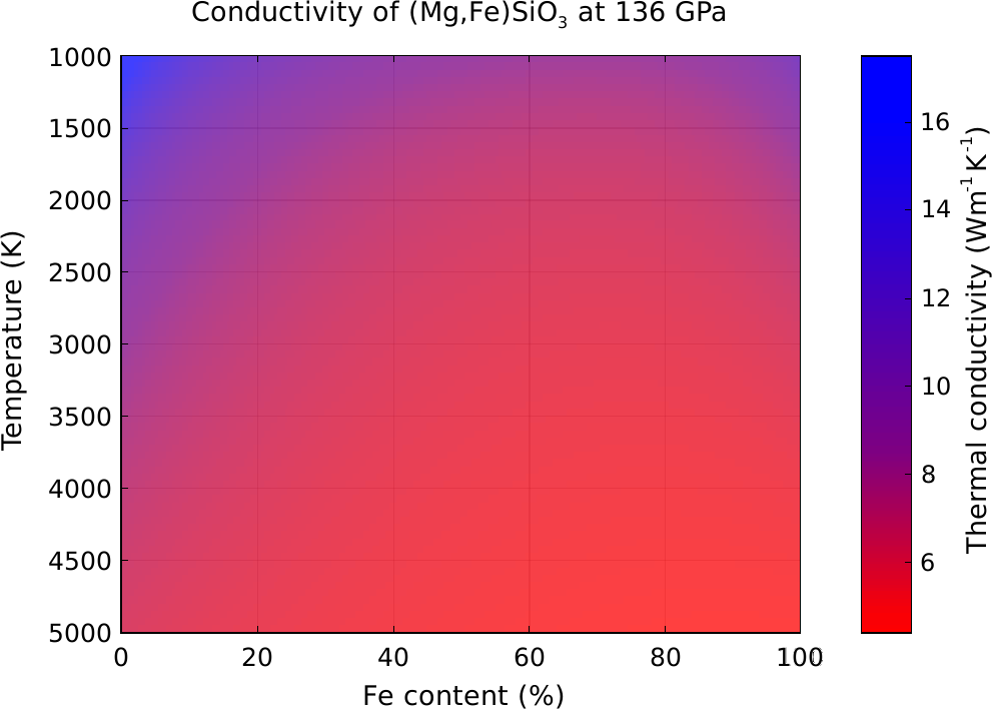
\includegraphics[width=\linewidth]{Figures/K_over_T_over_X.png}
  \caption{CAPTION}
  \label{fig:kappa-temp-comp_01}
\end{figure}












\pagebreak